% Тип документа
\documentclass[a4paper,12pt]{extarticle}

% Шрифты, кодировки, символьные таблицы, переносы
\usepackage{cmap}
\usepackage[T2A]{fontenc}
\usepackage[utf8x]{inputenc}
\usepackage[russian]{babel}
\usepackage[table]{xcolor}
% Это пакет -- хитрый пакет, он нужен но не нужен
\usepackage[mode=buildnew]{standalone}

\usepackage
	{
		% Дополнения Американского математического общества (AMS)
		amssymb,
		amsfonts,
		amsmath,
		amsthm,
		physics,
		% misccorr,
		% 
		% Графики и рисунки
		wrapfig,
		wasysym,
		graphicx,
		subcaption,
		float,
		tikz,
		tikz-3dplot,
		caption,
		csvsimple,
		color,
		booktabs,
		pgfplots,
		pgfplotstable,
		geometry,
		% 
		% Таблицы, списки
		array,
		makecell,
		multirow,
		indentfirst,
		%
		% Интегралы и прочие обозначения
		ulem,
		esint,
		esdiff,
		% 
		% Колонтитулы
		fancyhdr,
	}  

\usepackage{xcolor}
\usepackage{hyperref}

 % Цвета для гиперссылок
\definecolor{linkcolor}{HTML}{000000} % цвет ссылок
\definecolor{urlcolor}{HTML}{799B03} % цвет гиперссылок
 
\hypersetup{pdfstartview=FitH,  linkcolor=linkcolor,urlcolor=urlcolor, colorlinks=true}
% Обводка текста в TikZ
\usepackage[outline]{contour}

% Увеличенный межстрочный интервал, французские пробелы
\linespread{1.1} 
\frenchspacing 

 
\usetikzlibrary
	{
		decorations.pathreplacing,
		decorations.pathmorphing,
		patterns,
		calc,
		scopes,
		arrows,
		fadings,
		through,
		shapes.misc,
		arrows.meta,
		3d,
		quotes,
		angles,
		babel
	}

\usepgfplotslibrary{units}

% const прямым шрифтом
\newcommand\ct[1]{\text{\rmfamily\upshape #1}}
\newcommand*{\const}{\ct{const}}
\renewcommand*{\epsilon}{\varepsilon}

\usepackage[europeanresistors,americaninductors]{circuitikz}

% Style to select only points from #1 to #2 (inclusive)
\pgfplotsset{select/.style 2 args={
    x filter/.code={
        \ifnum\coordindex<#1\def\pgfmathresult{}\fi
        \ifnum\coordindex>#2\def\pgfmathresult{}\fi
    }
}}

\usepackage{array}
\usepackage{pstool}

%%%%%%%%%%%%%%%%%%%%%%%%%%%%%%%%%%%%%%%%%%%%%%%%%
\makeatletter
\newif\if@gather@prefix 
\preto\place@tag@gather{% 
  \if@gather@prefix\iftagsleft@ 
    \kern-\gdisplaywidth@ 
    \rlap{\gather@prefix}% 
    \kern\gdisplaywidth@ 
  \fi\fi 
} 
\appto\place@tag@gather{% 
  \if@gather@prefix\iftagsleft@\else 
    \kern-\displaywidth 
    \rlap{\gather@prefix}% 
    \kern\displaywidth 
  \fi\fi 
  \global\@gather@prefixfalse 
} 
\preto\place@tag{% 
  \if@gather@prefix\iftagsleft@ 
    \kern-\gdisplaywidth@ 
    \rlap{\gather@prefix}% 
    \kern\displaywidth@ 
  \fi\fi 
} 
\appto\place@tag{% 
  \if@gather@prefix\iftagsleft@\else 
    \kern-\displaywidth 
    \rlap{\gather@prefix}% 
    \kern\displaywidth 
  \fi\fi 
  \global\@gather@prefixfalse 
} 
\newcommand*{\beforetext}[1]{% 
  \ifmeasuring@\else
  \gdef\gather@prefix{#1}% 
  \global\@gather@prefixtrue 
  \fi
} 
\makeatother
%%%%%%%%%%%%%%%%%%%%%%%%%%%%%%%%%%%%%%%%%%%%%%%%%

\geometry		
	{
		left			=	2cm,
		right 			=	2cm,
		top 			=	3cm,
		bottom 			=	3cm,
		bindingoffset	=	0cm
	}

%%%%%%%%%%%%%%%%%%%%%%%%%%%%%%%%%%%%%%%%%%%%%%%%%%%%%%%%%%%%%%%%%%%%%%%%%%%%%%%

	%применим колонтитул к стилю страницы
\pagestyle{fancy} 
	%очистим "шапку" страницы
\fancyhead{} 
	%слева сверху на четных и справа на нечетных
\fancyhead[R]{\labauthors} 
	%справа сверху на четных и слева на нечетных
\fancyhead[L]{Отчёт по лабораторной работе №\labnumber} 
	%очистим "подвал" страницы
\fancyfoot{} 
	% номер страницы в нижнем колинтуле в центре
\fancyfoot[C]{\thepage} 

%%%%%%%%%%%%%%%%%%%%%%%%%%%%%%%%%%%%%%%%%%%%%%%%%%%%%%%%%%%%%%%%%%%%%%%%%%%%%%%

\renewcommand{\contentsname}{Оглавление}

\usepackage{tocloft}
% \renewcommand{\cftpartleader}{\cftdotfill{\cftdotsep}} % for parts
% \renewcommand{\cftsectiondotsep}{\cftdotsep}% Chapters should use dots in ToC
\renewcommand{\cftsecleader}{\cftdotfill{\cftdotsep}}
%\renewcommand{\cftsecleader}{\cftdotfill{\cftdotsep}} % for sections, if you really want! (It is default in report and book class (So you may not need it).
% ---------
% \newcommand{\cftchapaftersnum}{.}%
% \usepackage{titlesec}
% \titlelabel{\thetitle.\quad}
\usepackage{secdot}
\sectiondot{subsection}
\newcommand{\rot}{\operatorname{rot}}
\begin{document}

\def\labauthors{Виноградов И.Д., Понур К.А., Шиков А.П.}
\def\labgroup{0420ДМР1Г}
\def\labnumber{1}
\def\labtheme{Исследование рабочих характеристик оптимального обнаружителя сложных радиолокационных сигналов.}

\begin{titlepage}

\begin{center}

{\small\textsc{Нижегородский государственный университет имени Н.\,И. Лобачевского}}
\vskip 1pt \hrule \vskip 3pt
{\small\textsc{Радиофизический факультет. Кафедра Радиотехники.}}

\vfill

{\Large Отчет по лабораторной работе №\labnumber\vskip 12pt\bfseries \labtheme}
	
\end{center}

\vfill
	
\begin{flushright}
	{Выполнили студенты группы \labgroup\\\ \labauthors}%\vskip 12pt Принял:\\ Менсов С.\,Н.}
\end{flushright}
	
\vfill
	
\begin{center}
	Нижний Новгород, \the\year
\end{center}

\end{titlepage}



\section{Введение}
Целью лабораторной работы является изучение работы оптимального приемника сложного
радиолокационного сигнала с помощью математической модели, реализованной в среде графического
программирования LabVIEW. В работе были исследованы спектральные и корреляционные
характеристики импульса с линейной частотной модуляцией. Также экспериментальным путем
были получены рабочие характеристики приемника, оптимизированного для обнаружения на
фоне белого Гауссова шума полностью известного сигнала. Затем те же измерения были
выполнены для сигнала со случайной фазой и амплитудой (а также со случайной фазой
и случайной амплитудой одновременно). В ходе работы была симулирована работа приемника
сложных сигналов, были изучены оптимальные реализации эксперимента, когда приемник
настраивался верно (при этом количество правильных обнаружений было гораздо больше
количества ложных тревог).

Стоит отметить, что в ходе лабораторной работы нами был освоен пользовательский интерфейс
программы в среде графического программирования LabVIEW и как следствие были отточены
навыки работы с этой программой. Программа Laba\_SRS.vi (RADAR), содержащая эмулированную версию
экспериментальной установки, запускалась с помощью персонального компьютера.
Соответственно, все вычислительные работы производились с использованием ресурсов
персонального компьютера.

В современных радиотехнических системах широко применяется цифровая обработка сигналов.
В данной работе будет исследоваться упрощенная модель, описывающая только основные этапы
алгоритма оптимальной обработки радиолокационного сигнала, которые следуют за его
оцифровкой. Такая обработка может быть реализована как с помощью специализированных
сигнальных процессоров, так и с помощью компьютера общего назначения с соответствующим
программным обеспечением. Эта модель не включает такие важные этапы обработки,
как усиление и предварительную фильтрацию сигнала, его перенос на промежуточную
частоту, окончательную фильтрацию, автоматическую регулировку усиления и другие
адаптивные процедуры. В ней также не отражены систематические изменения амплитуды
сигнала, вызванные, например, прохождением цели через диаграмму направленности
антенны. Не учтен в модели и доплеровский сдвиг частоты, возникающий при движении
цели. Тем не менее, предлагаемая модель позволяет без использования реальной
аппаратуры получить хорошее представление о процессах обработки сигналов в
радиолокационных системах, которые происходят после переноса сигнала на
промежуточную частоту, фильтрации и оцифровки.


% \subsection{Задание 1}
% \textit{В начале отчета привести блок- схемы оптимального приемника
% радиолокационного сигнала с использованием корреляторов и
% согласованного фильтра, объяснить назначение их элементов. Привести
% теоретические формулы для РХП в случае обнаружения известного
% сигнала и сигнала со случайной фазой и амплитудой.}


Согласованный фильтр — это линейный оптимальный фильтр, построенный исходя из известных
спектральных характеристик полезного сигнала и шума. Согласованные фильтры предназначены
для выделения сигналов известной формы на фоне шумов. Под оптимальностью понимается
максимальное отношение сигнал/шум на выходе фильтра, и так как фильтр линейный форма
сигнала на выходе остается неизменной.


% \begin{figure}[h!]
% 	\centering
% 	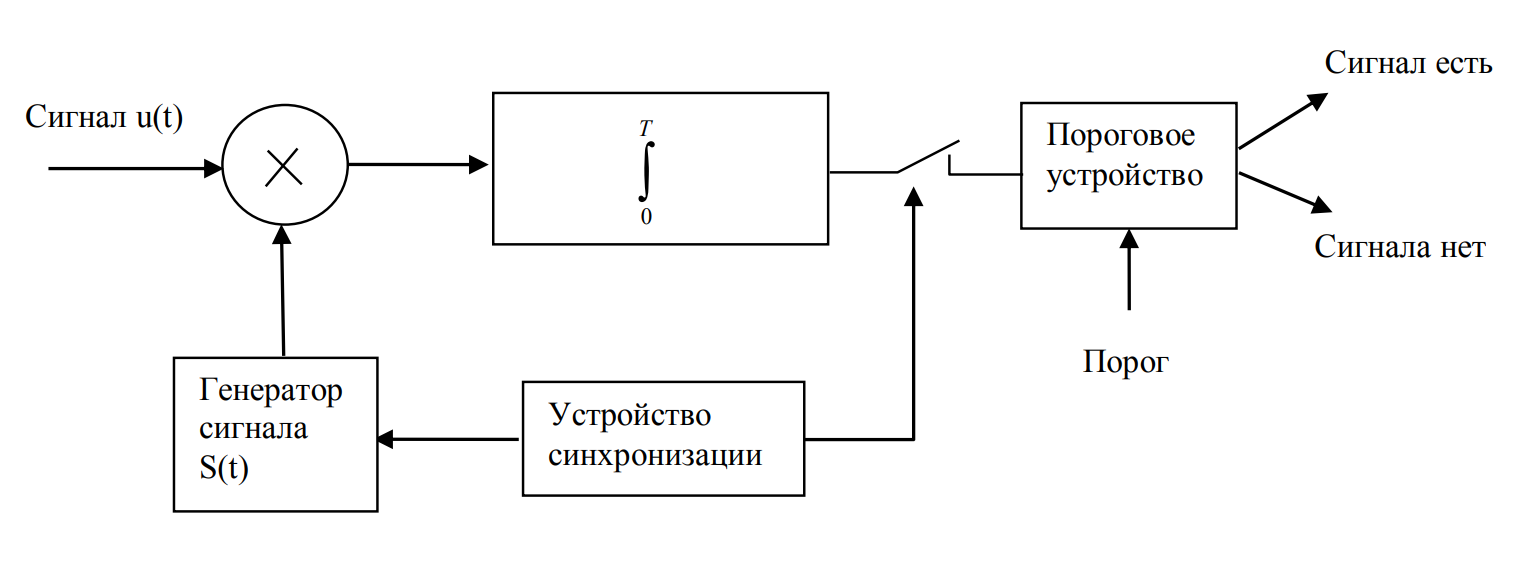
\includegraphics[width =0.8\linewidth]{imgs/scheme1.png}
% 	\caption{Блок-схема оптимального обнаружителя известного сигнала на фоне белого гауссова
%     шума}
% 	\label{fig:scheme1}
% \end{figure}

Для радио- и гидролокационных систем момент появления отраженного
сигнала, как правило, неизвестен. У отраженного от реальной цели сигнала фаза, а
также амплитуда, являются случайными величинами. Теоретический вид оптимального
приемника с использованием корреляторов приведен на рис. \ref{fig:scheme2}.

Такой приемник включает два идентичных коррелятора, на которые в
качестве опорных подаются излучаемый сигнал и его квадратура. На выходах
корреляторов формируются действительная I и мнимая Q составляющие
некоторого аналитического сигнала. На пороговое устройство подается его
огибающая. 
Пороговое устройство фильтрует сигнал в зависимости от амплитуды выходного сигнала.

Упрощенную схему можно реализовать с
помощью согласованного фильтра, как это показано на рис. \ref{fig:scheme3}.

\begin{figure}[h!]
	\centering
	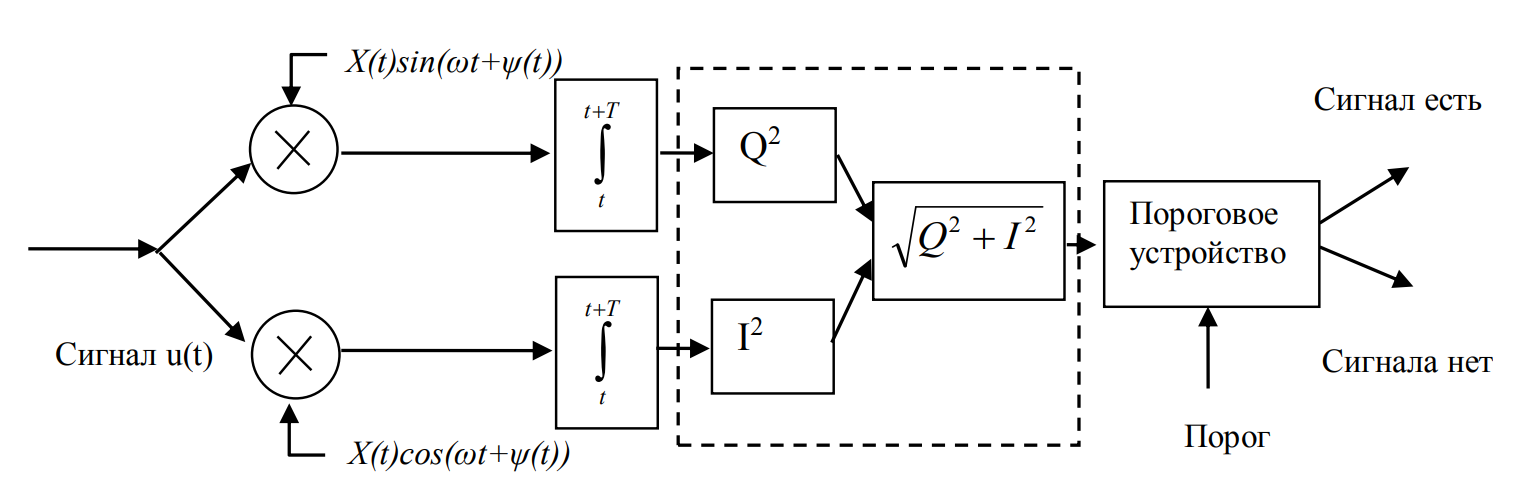
\includegraphics[width =0.8\linewidth]{imgs/scheme2.png}
	\caption{Блок-схема обнаружителя сигнала со случайной фазой и амплитудой на фоне белого
    гауссова шума с использованием двух корреляторов (устройство синхронизации на данной
    схеме отсутствует, т.к. интегрирование ведется в скользящем окне)
    }
	\label{fig:scheme2}
\end{figure}

\begin{figure}[h!]
	\centering
	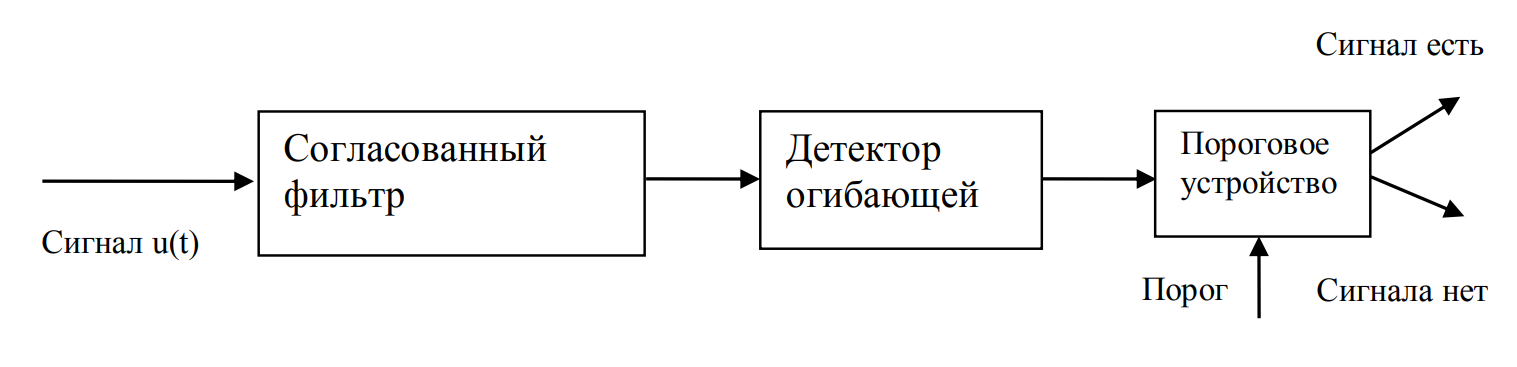
\includegraphics[width =0.8\linewidth]{imgs/scheme3.png}
	\caption{Блок-схема обнаружителя сигнала со случайной фазой и амплитудой на фоне
    белого гауссова шума с использованием согласованного фильтра и детектора огибающей}
	\label{fig:scheme3}
\end{figure}

Детектор огибающей осуществляет измерение огибающей входного сигнала,
т.е. формирует выходной сигнал вида $u_{\text{вых}}(t) = K_{\text{дет}}A(t)$.

Для выбора порога $l_0$ в задаче обнаружения в радио- и акустической
локации применяется критерий Неймана-Пирсона. Он гласит, что
при заданном отношении сигнал/шум порог должен выбираться так, чтобы при
фиксированной величине вероятности ложной тревоги $P_\text{ЛТ}$ вероятность $P_\text{ПО}$ правильного
обнаружения была максимальной. Связь между этими вероятностями
называется рабочей характеристикой приемника - \textbf{РХП}.
 
Для обнаружителя детерминированного сигнала на фоне белого гауссова шума РХП получается только в параметрическом виде,
где параметром выступает порог обнаружения $l_0$:
\begin{equation}
    P_\text{ПО} = 1- F\left(\frac{\ln(l_0)}{d} - d/2\right), \quad
    P_\text{ЛТ} = 1 - F\left(\frac{\ln(l_0)}{d} + d/2\right),
    \label{eq:laplace}
\end{equation}
где $P_\text{ПО}$ - вероятность правильного обнаружения, $P_\text{ЛТ}$ - вероятность ложной тревоги,
$F(x) = \frac{1}{\sqrt{2\pi}}\int\limits_{-\infty}^{x}\exp(-y^2/2)\dd y$ - интеграл Лапласа,
$d^2 = 2 E/N_0$ - отношение энергии сигнала к спектральной плотности мощности (СПМ) шума. 

При неизвестной фазе выражение для РХП имеет вид
\begin{equation}
    P_\text{ПО} = Q(d, \sqrt{2 \ln(1/P_\text{ЛТ})}).
    \label{eq:marqum}
\end{equation}
Здесь  $Q(v,u) = \int \limits_{u}^{\infty} x I_0 (v x) \exp \left(-\frac{x^2 + y^2}{2}\right) \dd x$ - 
фунцкия Маркума.

Если случайными являются фаза и амплитуда, выражение для РХП примет следующий вид (при условии что
распределение амплитуды имеет вид Рэлеевского):
\begin{equation}
    P_\text{ПО} = P_\text{ЛТ}^{\frac{1}{1+d^2/2}}.
    \label{eq:theory}
\end{equation}

Для обнаружителя сигнала со случаной фазой нужно использовать два идентичных коррелятора
на которые в качестве опорных подается излучаемый сигнал и его квадратура. На выходах
корреляторов формируются действительная I и мнимая Q составляющие некоторого
аналитического сигнала.

\section{Практическая часть}


\subsection{Исследование спектра и корреляционной функции ЛЧМ-сигнала}
% \subsection{Задание 2. Спектр и корреляционная функция ЛЧМ-сигнала}
Было проведено сравнение спектра и корреляционной функции ЛЧМ-сигнала для окна с
плоской вершиной при различных значениях разности начальной чатсоты $f_{s}$ и
конечной частоты $f_{e}$. Полученные графики приведены на рис. \ref{fig:spec1}-\ref{fig:spec4}

\begin{figure}[H]
    \centering
    \begin{minipage}{0.49\linewidth}
        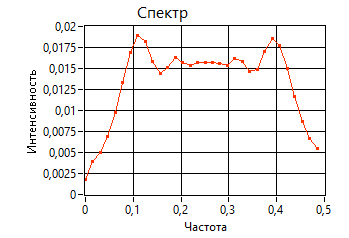
\includegraphics[width =0.9\linewidth]{imgs/spec1.png}
    \end{minipage}
    \begin{minipage}{0.49\linewidth}
        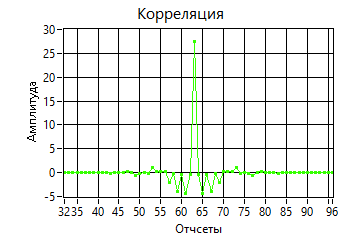
\includegraphics[width =0.9\linewidth]{imgs/corr1.png}
    \end{minipage}
	\caption{Разница частот 0.5 ($f_{s}=0, f_{e}=0.5$). Разница фаз = 0}
	\label{fig:spec1}
\end{figure}

\begin{figure}[H]
    \centering
    \begin{minipage}{0.49\linewidth}
        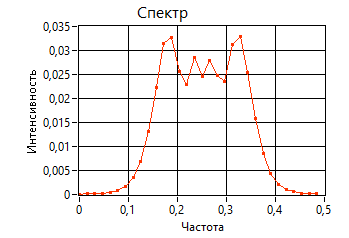
\includegraphics[width =0.9\linewidth]{imgs/spec2.png}
    \end{minipage}
    \begin{minipage}{0.49\linewidth}
        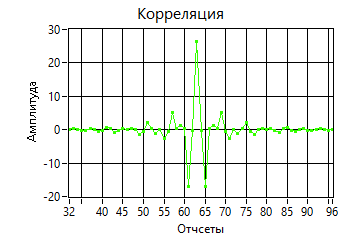
\includegraphics[width =0.9\linewidth]{imgs/corr2.png}
    \end{minipage}
	\caption{Разница частот 0.3 ($f_{s}=0.1, f_{e}=0.4$). Разница фаз = 0}
	\label{fig:spec2}
\end{figure}

\begin{figure}[H]
    \centering
    \begin{minipage}{0.49\linewidth}
        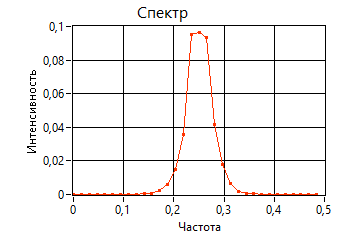
\includegraphics[width =0.9\linewidth]{imgs/spec3.png}
    \end{minipage}
    \begin{minipage}{0.49\linewidth}
        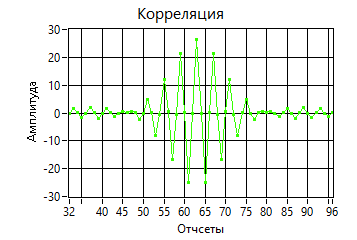
\includegraphics[width =0.9\linewidth]{imgs/corr3.png}
    \end{minipage}
	\caption{Разница частот 0.1 ($f_{s}=0.2, f_{e}=0.3$). Разница фаз = 0}
	\label{fig:spec3}
\end{figure}

\begin{figure}[H]
    \centering
    \begin{minipage}{0.49\linewidth}
        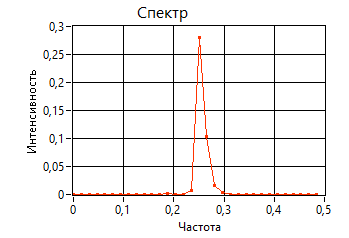
\includegraphics[width =0.9\linewidth]{imgs/spec4.png}
    \end{minipage}
    \begin{minipage}{0.49\linewidth}
        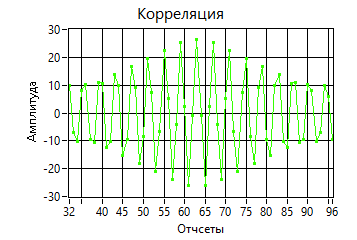
\includegraphics[width =0.9\linewidth]{imgs/corr4.png}
    \end{minipage}
	\caption{Разница частот 0.01 ($f_{s}=0.25, f_{e}=0.26$). Разница фаз = 0}
	\label{fig:spec4}
\end{figure}

Из полученных результатов видно, что при уменьшении разницы между начальной
и конечной частотой ширина корреляционной функции увеличивается, ширина спектра уменьшается,
а значение базы сигнала уменьшается.

Очевидно, что при  изменении частотной полосы ЛЧМ-сигнала его спектр
пропорционально увеличивается. Исследуемый сигнал является стационарным в
широком смысле случайным процессом, а значит его спектр связан с корреляционной
функцией обратным преобразованием Фурье:

\begin{equation}
    K(\tau) = \int\limits_{-\infty}^{\infty} S(\omega) \exp{+j\omega\tau} \dd{\omega}
\end{equation}

А для пары преобразований Фурье мы можем написать соотношение неопределенности
в виде:
\begin{equation}
    \Delta \tau  \Delta \omega \geq 2\pi, \text{ где}
\end{equation} 

$\Delta \omega$ -- характерная ширина спектра, $\Delta \tau$ -- характерное время корреляции.

Уменьшенеие ширины спектра объясняется уменьшением количества частотных компонент, использованных 
в сигнале. Таким образм, при устремлении разницы частот к нулю, вид спектра будет приближаться к $\delta$-функции.


% \subsection{Задание 3. Исследование РХП}
\subsection{Исследование РХП}
Зависимости вероятности правильного
обнаружения $P_\text{ПО}$ от вероятности ложной тревоги $P_\text{ЛТ}$ для трех значений
отношения сигнал/шум были изучены для следующих сигналов: детерминированный, со случайной фазой,
со случайной амплитудой, со случайными фазой и амплитудой. Использовались значения СКО шума $0.25, 0.5, 1, 1.5$.
Результаты приведены на рис. \ref{fig:task3}.

Как и ожидалось, график РХП для детерминированного сигнала имеет достаточно резкий вид по сравнению
с другими сигналами, поскольку отсутствуют случайные компоненты.
Сигнал со случайной фазой также имеет достаточно резкую форму графика РХП.

Сигнал со случайной амплитудой и случайной фазой имеет более плавную зависимость, поскольку
большая часть случаев ложных тревог и пропусков цели зависит именно от амплитуды, которая в данном случае случайна.

Были рассчитаны теоретические зависимости РХП для разных сигналов.
Для детерминированного сигнала в качестве теоретических использовались формулы \eqref{eq:laplace},
 отношение сигнал/шум, входящее в эту формулу получалось
 экспериментально для каждого сигнала и значения СКО.
$\text{SNR} = E/N_0$, где $\text{SNR}$ -
% энергия сигнала рассчитывалась как
% $E=0.5 A^2 \tau_i$ ($A$ - амплитуда сигнала, $\tau_i$ - длительность импульса), а СПМ  шума как $N_0=$

В случае сигнала со случайной амплитудой использовалась функция Маркума \eqref{eq:marqum} 
(при вычислении использовался интеграл от распределения Райса), а для сигнала со случайной амплитудой и фазой
использовалась формула \eqref{eq:theory}. Соответствующие теоретические зависимости также приведены на \ref{fig:task3}.

По приведенным результатам видно, что экспериментальные зависимости по характеру совпадают с теоретическими,
однако отличаются абсолютными значениями.

На графиках \ref{fig:task3} также отмечены точки для одинакового значения величины порога $l_0$: $\triangle - 20, \square - 10, \ocircle - 3$.

Наблюдается общая закономерность - чем больше значение порога, тем меньше вероятность
ложной тревоги и меньше вероятность правильного обнаружения.

Сравнивая графики для 
различных сигналов, можно сделать вывод, что при одинаковых значениях порога вероятность правильного
обнаружения уменьшается по сравнению с детерминированным сигналом.
Сильнее всего это выражено для сигналов со случайной амплитудой, в то время как для сигнала
со случайной фазой зависимость вероятности правильного обнаружения от величины порога близка
к зависимости для детерминированного сигнала.

На графике \ref{fig:task3} также отмечены точки для одинакового значения порога $l_0$: $\triangle - 3, \square - 10, \ocircle - 20$.

\begin{figure}[H]
    \centering
    \begin{subfigure}{0.49\linewidth}
        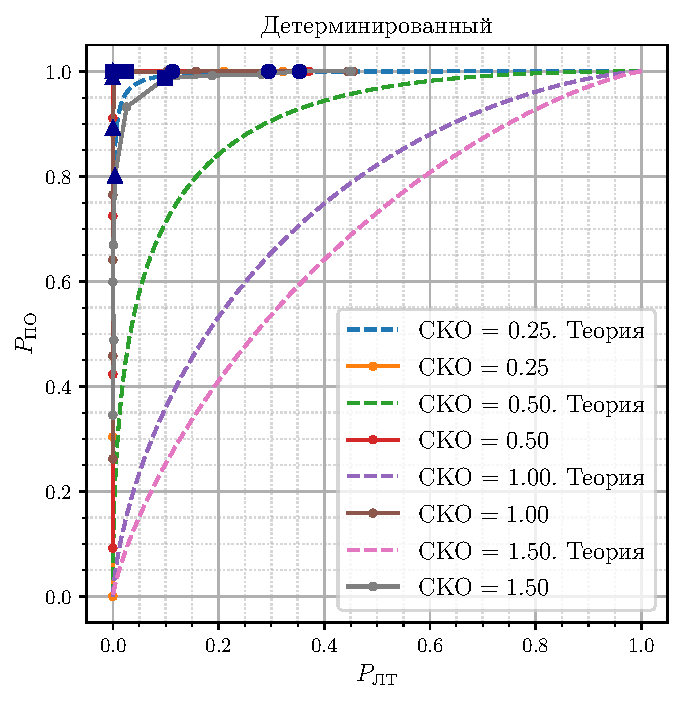
\includegraphics[width=\linewidth]{data/data_determ.pdf}
    \end{subfigure}
    \begin{subfigure}{0.49\linewidth}
        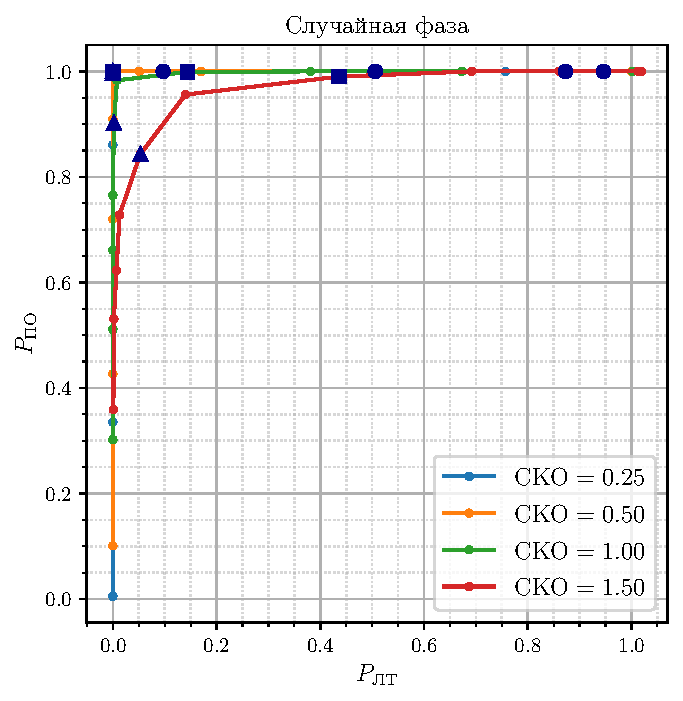
\includegraphics[width=\linewidth]{data/data_phase.pdf}
    \end{subfigure}
\end{figure}
\begin{figure}[H]
    \centering
    \begin{subfigure}{0.49\linewidth}
	    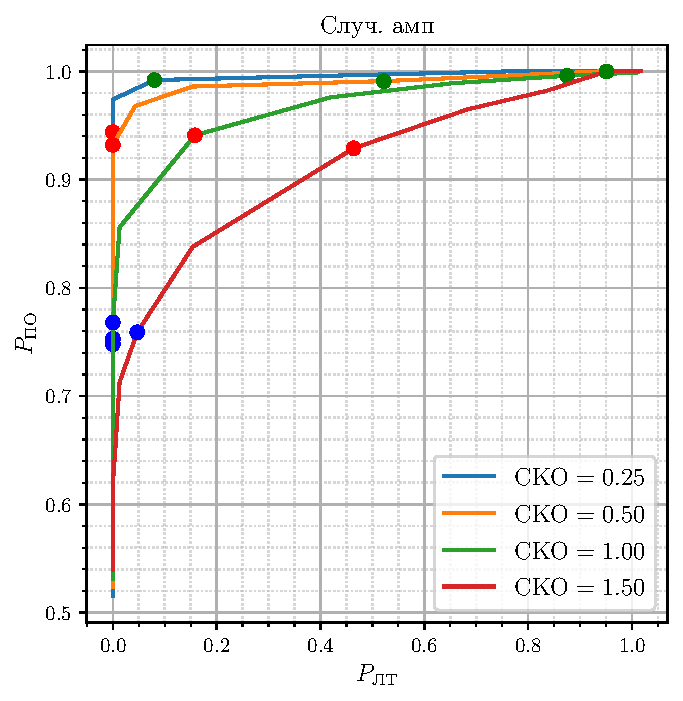
\includegraphics[width=\linewidth]{data/data_amplitude.pdf}
    \end{subfigure}
    \begin{subfigure}{0.49\linewidth}
	    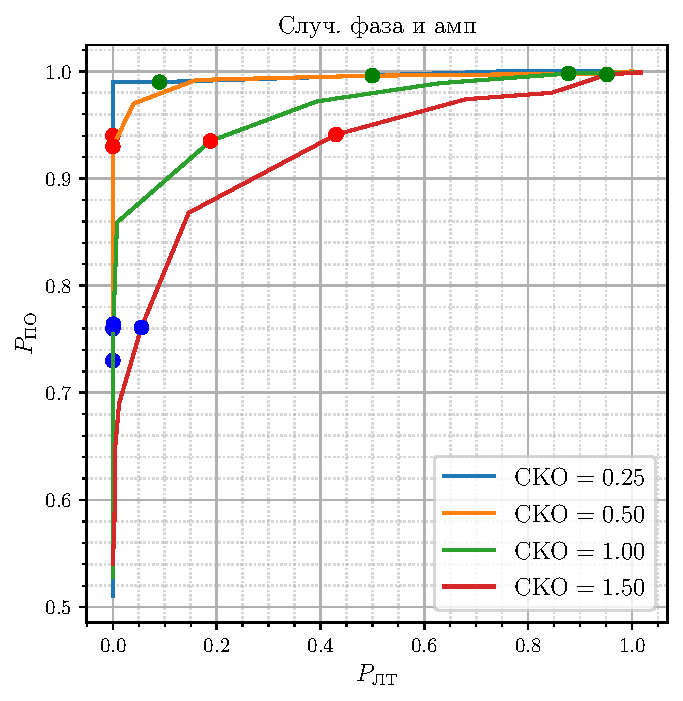
\includegraphics[width=\linewidth]{data/data_phase_amplitude.pdf}
    \end{subfigure}
    \caption{Графики зависимости РХП для различных сигналов и различных значений СКО. Пунктирными линиями 
    отмечены теоретические зависимости для соответствующего сигнала.
    На графиках также отмечены одинаковые значения порога: $\triangle - 3, \square - 10, \ocircle - 20$.}
    \label{fig:task3}
\end{figure}

\section{Вывод}

\end{document}
